%Scientific application workflows properties, such as size, and requirements, such 
%as type and number of resources, change in time. In scientific campaign
%
%These properties of the workflow are not necessarily captured during the 
%specification of the workload. 
%
%bla bla workload manager autonomic IBM~\cite{ibm2005autonomic}

% ------------------------------------------------------------------------------
% Scientific campaings
\gpnote{Campaings and workflow characteristics. Refer to the workflows from 
ICEBERG and Oliver and constraint the problem there.}
Ensemble based scientific campaigns execute ensembles of pipelines with 
heterogenoues characteristics and requirements. These pipelines can be single 
branched~\cite{paraskevakos2019workflow,dakka2018high,ramakrishnan_survey,
balasubramanian2018harnessing} to pipelines with complex data and control 
dependencies~\cite{ramakrishnan_survey,deelman2018future}. Futhrermore, they 
can be static~\cite{paraskevakos2019workflow} or dynamic~\cite{dakka2018high,
balasubramanian2018harnessing}. Dynamicity in pipelines is realizd via control 
loops, where new stages are added, while in campaigns by adding ensemble 
members during runtime.

Pipelines from Biomolecular and Earth sciences are mainly single branched. 
Biomolecular pipelines may present adaptivity by adding additional stages after 
some analysis step. Earth science pipelines are mostly static, but they may 
have $\mathcal{O}(10k)$ to $\mathcal{O}(100k)$ ensemble members. In this work, 
we will initially assume that the workflow, and its pipelines are static. In 
addition, we will assume that the workflow has enough ensemble members, such 
that it cannot be run in a single job on HPC. Next, we are going to relax this 
assumption, and assume that the pipelines are adaptive.

% ------------------------------------------------------------------------------
% Workflow modeling
\gpnote{
\begin{enumerate}
\item We initially know the distribution
\item Then relax assumption about distributions, task size, static/dynamic
\item Transform the model to a question: This can be amenable to different type 
of model from an experimental model to a formal queuing theory model
 \end{enumerate}}

Predicting the execution time of the whole or part of the workflow at any stage 
of the campaign's execution is necessary for correct planning. As a result, 
having performance modeling is necessary. Workflows have been modeled by using 
queueing theory~\cite{bao2019performance,yao2019throughput}, machine 
learning~\cite{witt2019predictive,pumma2017runtime}, domain specific 
languages~\cite{deelman2017performance,mandal2016toward}, markov decision 
processes~\cite{jia2005cost}. 

\begin{figure*}[ht!]
    \centering
    \begin{subfigure}[b]{0.25\textwidth}
        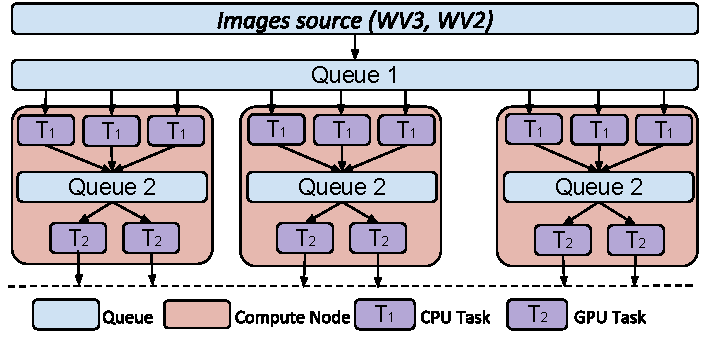
\includegraphics[width=\linewidth]{figures/SealsDesign2.pdf}
        \caption{Earth Sciences example workflow}
    \end{subfigure}%
    ~ 
    \begin{subfigure}[b]{0.25\textwidth}
        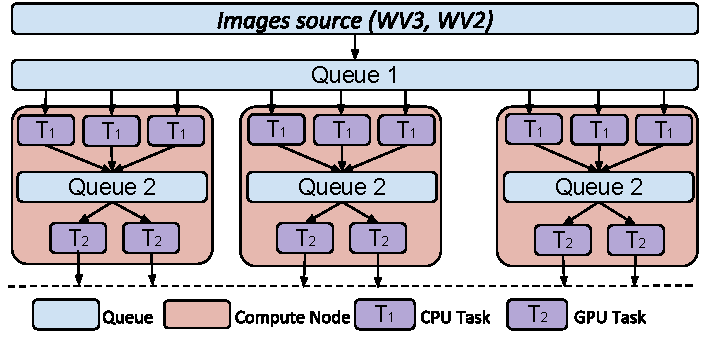
\includegraphics[width=\linewidth]{figures/SealsDesign2.pdf}
        \caption{Biomolecular Sciences example workflow}
    \end{subfigure}
    \caption{Simple Architectural Diagram. The Application Manager through 
    EnTK's API receives a workflow, a resource request, and a deadline and 
    communicates to the Autonomic Tuner. Autonomic Tuner, based on information 
    in Knowledge Base makes a decision and passes it to the Resource Manager. 
    Based on information of the execution state of the workflow the Autonomic 
    Tuner updates the knowledge base and its decision}\label{fig:bio_earth_workflows}
\end{figure*}

Biomolecular and earth science workflow can be modeled as queuing systems. Figure~\ref{fig:bio_earth_workflows} shows two basic workflows from biomolecular and earth sciences.

% ------------------------------------------------------------------------------
% Workflow management system


% ------------------------------------------------------------------------------
% Initial Assumptions

% ------------------------------------------------------------------------------
% Autonomic system makes sense
Monitoring, regulating, and configuring large scale scientific workflows 
require dedicated human resources that may not be available at any given point 
in time. Autonomic systems offer self-monitoring, self-configuring, and 
self-regulating capabilities. These capabilities can enable execute a 
scientific workflow on HPC resources without user intervention. Incorporated in 
a workflow management system a user can define a workflow, desired resources 
and expected time to completion. The workflow system will then be responsible 
to select how these resources will be used to execute the workflow in terms of 
concurrency, resource type (CPU, GPU) and walltime.

We propose creating an autonomic workload manager that will be able to offer 
these \textit{self-*} properties to scientific workflows. This middleware will 
be responsible in monitoring, configuring and regulating the execution based on 
policies and rules defined by the users.

Self-configuration is achieved by the software deciding the number of resources 
an execution will use to achieve a specific deadline. The middleware will take 
as input models for execution time, memory utilization, storage requirements of 
kernels used in the workflow. The distribution of the input dataset can also be 
provided. Based on models and a user's deadline it will make a decision how to 
configure the requested resources. That decision includes, but not limited to, 
number of cores, GPUs, type of memory size, and walltime.

Self-monitoring is achieved via the middleware being able to monitor and sample 
the execution state of the workflow. A state full workflow execution engine,
such as RADICAL-Enseble Toolkit~\cite{balasubramanian2018harnessing}, or 
Dask~\cite{rocklin2015dask}, is required. Such an engine allows the middleware 
to know the state of the workflow at any given point in time. This information 
can then be used to evaluate the configuration decision made.

Self-regulation is achieved by updating the decision during runtime to reflect 
knowledge obtained via monitoring. In addition, the decision making process is 
also updated. Based on the sampled state of execution, and the probability of 
achieving the defined goal, the system will adjust the execution of the 
workflow. If the initial decision was an underestimation, more resources can be 
added. When the decision was an overestimation, the heuristic can be updated 
such that less resources are used in a subsequent execution.

\gpnote{
\begin{enumerate}
    \item In design start speaking about machine, workflow style specific 
    models.
    \item The decision space depends on empirical space.
\end{enumerate}
}

A conceptual architecture is provided by Jha et al. in Ref.~\cite{jha2009self}. 
This architecture consists of a resource manager, an autonomic tuner and an 
application. It defines an Application objective, which is then translated to a 
set of measurable requirements, using well defined metrics, that the 
application should meet. These objectives are achieved through user defined 
mechanisms. Based on the objective and a set of mechanisms, the system can then 
define necessary strategies and actions to achieve the objective.

RADICAL-Ensemble Toolkit~\cite{balasubramanian2018harnessing} (EnTK) defines an 
application manager (AM), and a resource manager (RM). EnTK defines an 
application as a sequence of workflows that are executed. The workflows may 
either reuse resources or request new ones, based on how the user has 
programmed the application. In addition, the time requested for each resource 
is also decided by the user. The AM currently submits a workflow to the 
resources managed by RM and checks their overall execution state. In addition, 
the resource manager requests computing resource from an HPC and monitors their 
state. None of these components have any decision capabilities.

\begin{figure*}[t]
    \centering
    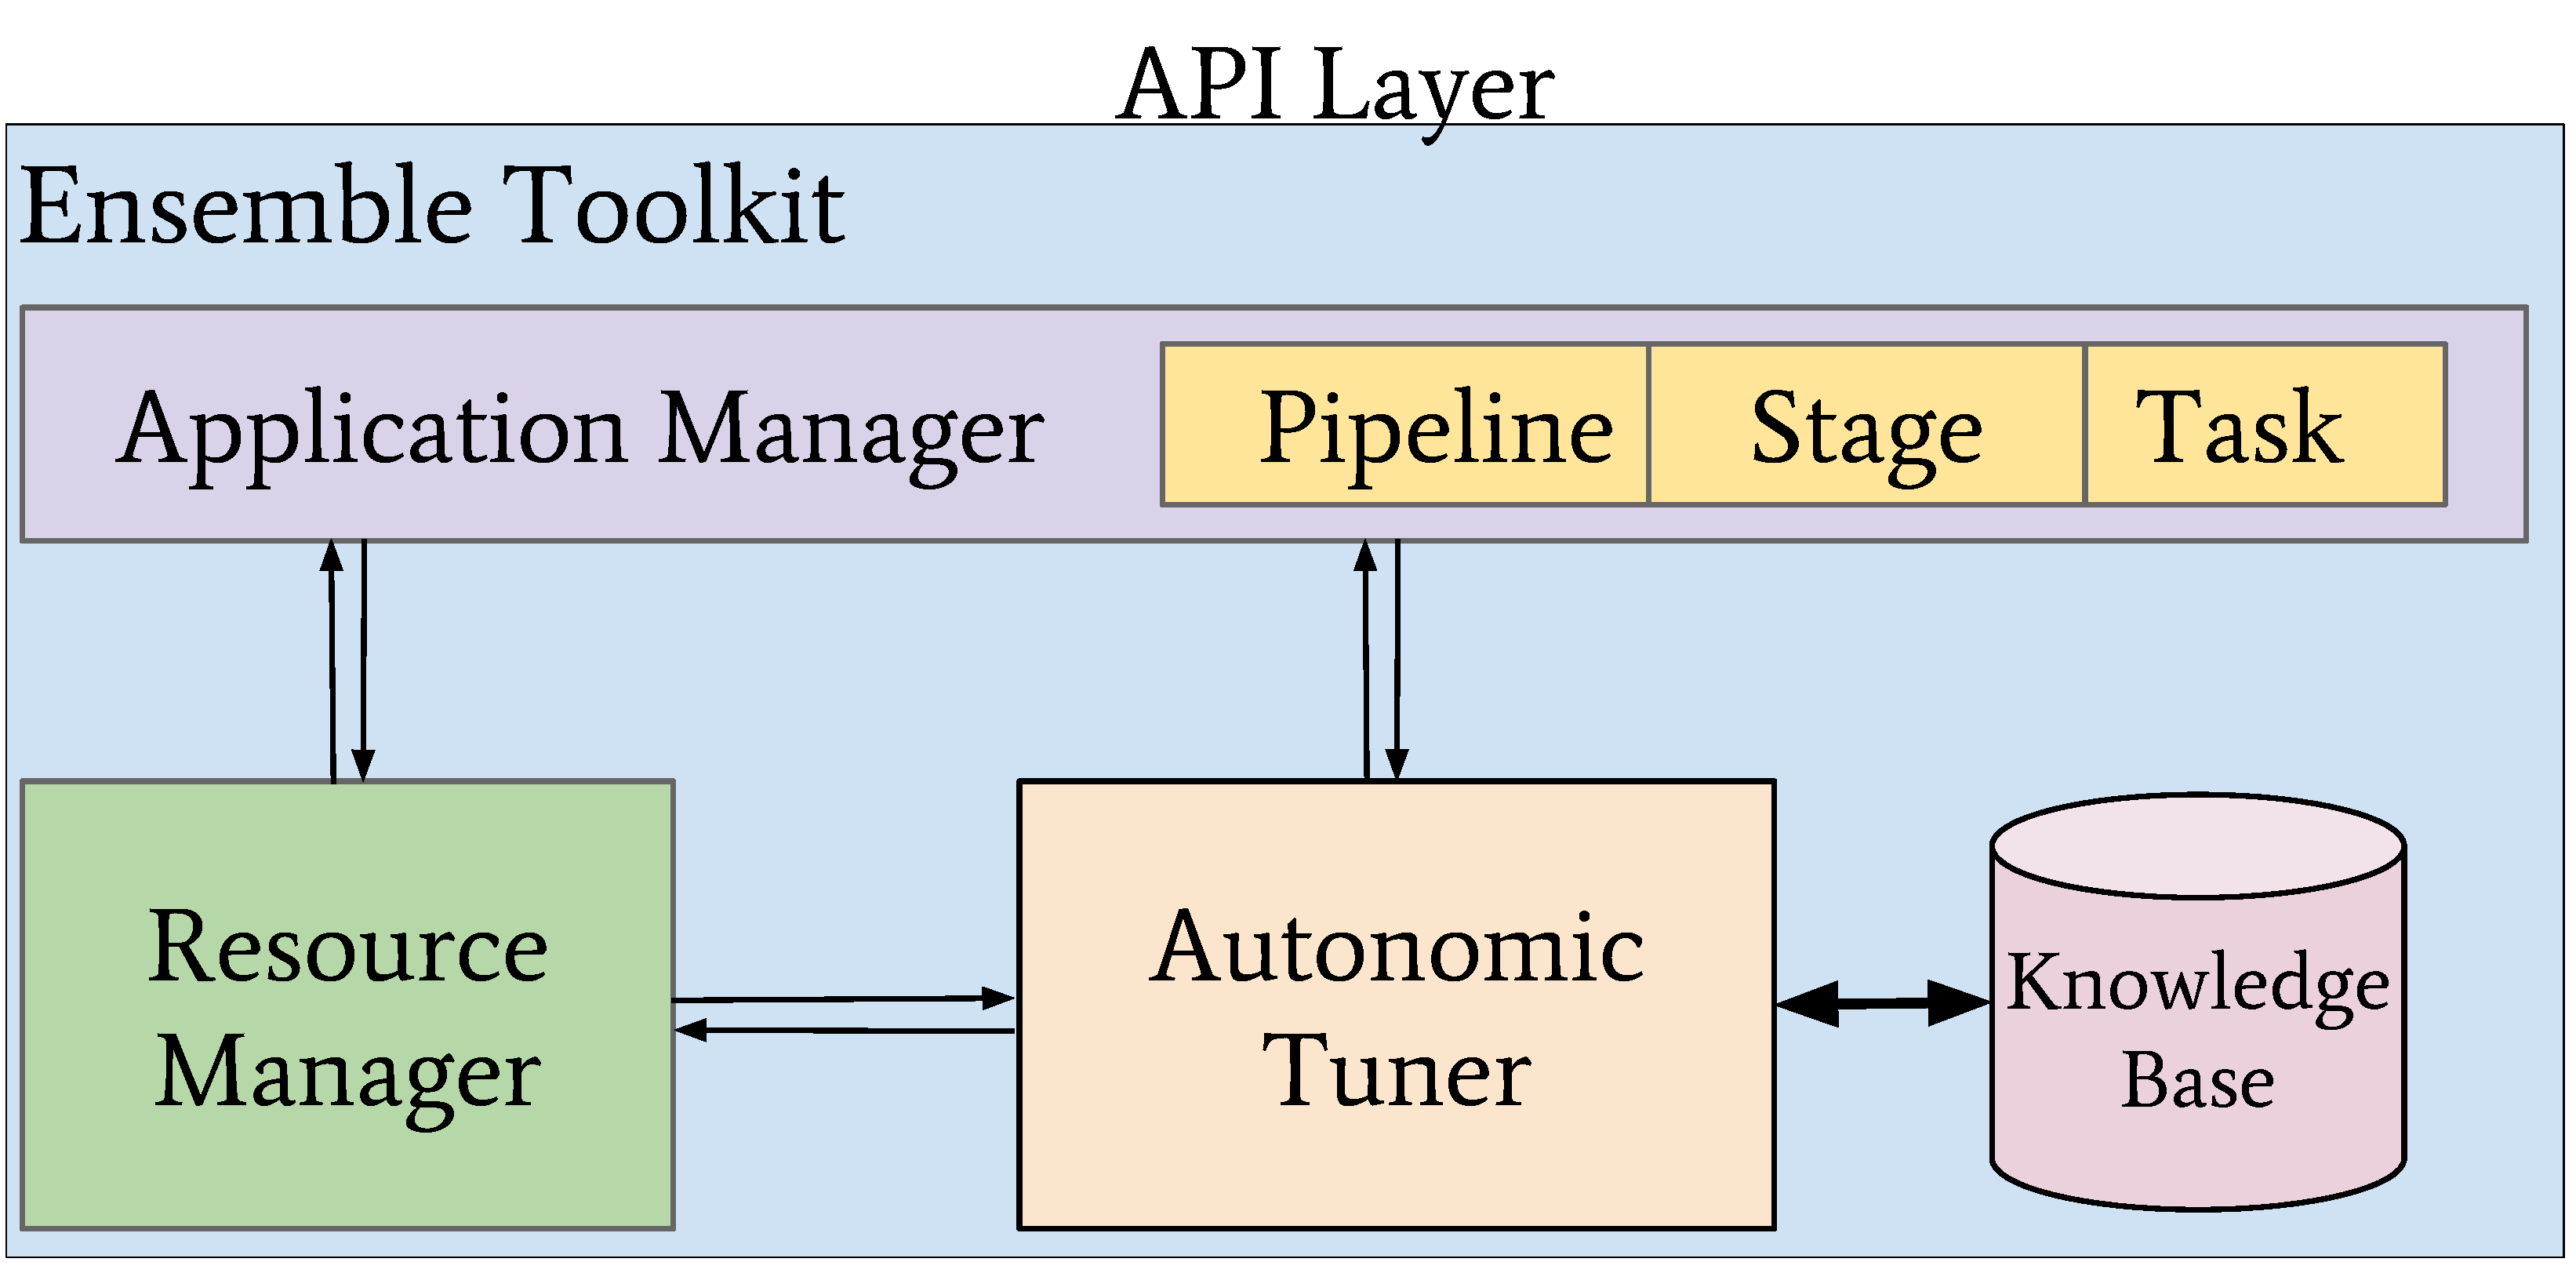
\includegraphics[width=.95\textwidth]{figures/AutonomicSubsystem.pdf}
    \caption{Simple Architectural Diagram. The Application Manager through 
    EnTK's API receives a workflow, a resource request, and a deadline and 
    communicates to the Autonomic Tuner. Autonomic Tuner, based on information 
    in Knowledge Base makes a decision and passes it to the Resource Manager. 
    Based on information of the execution state of the workflow the Autonomic 
    Tuner updates the knowledge base and its decision}\label{fig:architecture}
\end{figure*}


\gpnote{
\begin{enumerate}
\item After the architecture start discussing implementation. 
\item Since we are discussing about pilot jobs refer to RP and EnTK.
\end{enumerate}}

We propose to extend these two components of EnTK and introduce an autonomic 
tuner, as defined in Ref~\cite{jha2009self}. The AM, apart from the workflow 
definitions, can take as input information of the desired resources to execute 
the workflow, and an Application objective. Initially, the application 
objective could be as simple as an execution deadline, but it should be easily 
extansible to other metrics. The resource manager based on the desired 
resources can provide information about them, such maximum allowed node 
requests, maximum queue times, and more. The autonomic tuner, we propose to add,
 can use this information along with execution models for the workflow tasks to 
decide concurrency and timeline of the execution of the application. This 
achieves the self-configuration property of an autonomic system. The AM already 
monitors the execution state and it can report it to the tuner in specified 
intervals, achieving this way the self-monitoring property. The tuner then can 
decide whether more resources are required for achieving the deadline and 
update the decision rule, thus achieving the self-regulating aspect of an 
autonomic system. The resource manager acquires and monitors resource 
availability as they are needed by the tuner's decisions. In addition, the 
resource manager will provide information about which resources a workflow is 
executing. Figure~\ref{fig:architecture} shows a simple diagram of the 
architecture of the proposed extension. The Knowledge Base holds information 
such as execution models of the workflow, and historic data from previous 
executions.

Changing the number of resources used executing a workflow in HPC resources is 
not trivial. When more resources are required to a achieve a deadline, the 
workflow system through its autonomic capabilities can request as many 
computational nodes as needed.  On the other hand, when resources are 
underutilized, the autonomic system should either release part of them or 
update the decision for subsequent runs. Nodes on HPCs can be requested either 
as single or multiple nodes. Since many resources have policies at place to 
regulate the total number of concurrent jobs a user has, it is preferable to 
request nodes in numbers larger than one. That requires, whenever resources are 
released, to release them also as multiple nodes. Initially, we will assume 
that our workflows do not underutilize the resources.


\gpnote{Talk about EnTK's AppManager. See how an autonomic system controller 
can be added to extend it. It makes sense that each app manager will be able to 
decide it self about the execution of a workflow. }

